\documentclass[10pt,a4paper]{article}
\usepackage[utf8]{inputenc}
\usepackage{amsmath}
\usepackage{amsfonts}
\usepackage{amssymb}
\usepackage{multicol}
\usepackage{graphicx}
\usepackage{caption}
\usepackage{subcaption}
\usepackage{float}
\begin{document}

\section{2D lid-driven cavity}

Table \ref{tbl:part1} outlines the simulation settings for cases A - C of the lid driven cavity. Both the velocity and temperature fields at $t = 50$ are plotted in figures \ref{fig:1A} to \ref{fig:1C}. 

\begin{table}[H]
\centering
\begin{tabular}{c|cccccccc}
 & Re & $l_x$ & $l_y$& $T_{top}$ & $T_{bottom}$ & $N_x$ & $N_y$ & $\Delta t$ \\ 
\hline 
Case A & 20& 1 & 1  &0 & 1  & 30 & 30 & 0.001 \\ 

Case B & 200 & 1 & 1 & 0 & 1  & 50 & 50 & 0.001 \\ 
 
Case C & 4000 & 1 & 1 & 0 & 1  & 100 & 100 & 0.001 \\ 

\end{tabular} 
\caption{Simulation setting for 2D lid driven cavity.}
\label{tbl:part1}
\end{table}

\subsection{Case A}

\begin{figure}[H]
\centering
\begin{minipage}{.5\textwidth}
  \centering
  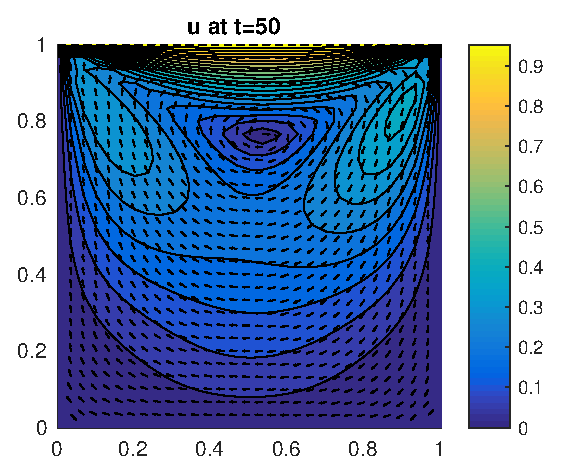
\includegraphics[width=.9\linewidth]{Part1_Case_A_Velocity.eps}
\end{minipage}%
\begin{minipage}{.5\textwidth}
  \centering
  \includegraphics[width=.9\linewidth]{Part1_Case_A_Temp.eps}
\end{minipage}
\caption{Case A: Velocity (left) and temperature (right) profiles at $t = 50$.}
\label{fig:1A}
\end{figure}

In case A the flow field is dominated by a primary vortex in the center of the domain. Some tell tale signs of low Reynolds number flow can be seen, primarily the symmetry of the velocity field resembling that of a Stokes solution. The passive scalar field also shows a slight deviation from the linear gradient imposed as an initial condition however very little indication of mixing can be seen at such low Reynolds number. The Neumann boundary condition enforced on the left and right sides is apart in the horizontal temperature contours.

\subsection{Case B}

\begin{figure}[H]
\centering
\begin{minipage}{.5\textwidth}
  \centering
  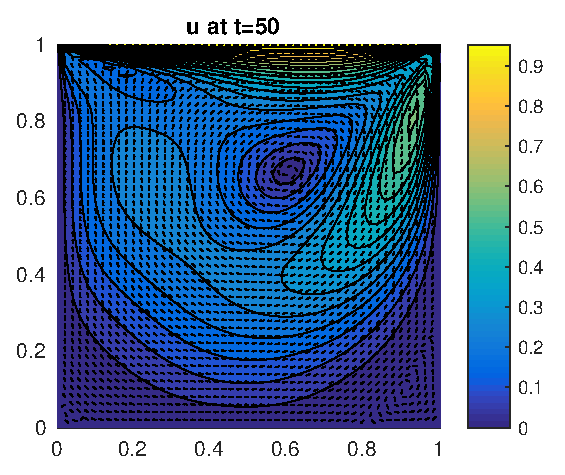
\includegraphics[width=.9\linewidth]{Part1_Case_B_Velocity.eps}
\end{minipage}%
\begin{minipage}{.5\textwidth}
  \centering
  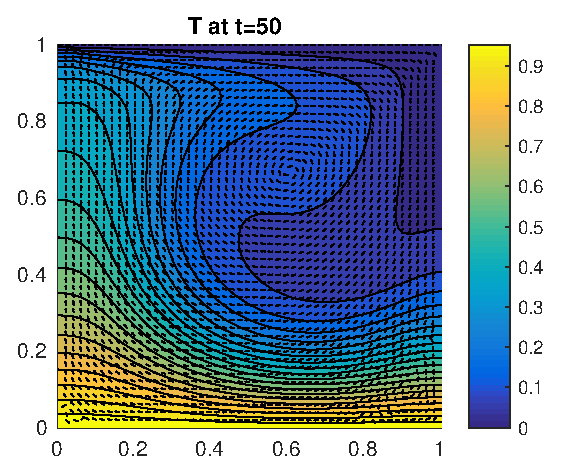
\includegraphics[width=.9\linewidth]{Part1_Case_B_Temp.eps}
\end{minipage}
\caption{Case B: Velocity (left) and temperature (right) profiles at $t = 50$.}
\label{fig:1B}
\end{figure}

In case B the flow field is still comprised of a single vortex however the impact of the advection term can be seen as this vortex is asymmetric. Higher velocities can be seen on the right side of the domain as the fluid is accelerated by the upper wall and forced into the right wall. This trend is matched in the passive scalar field indicating the low concentration on the upper surface being forced down on the right side of the domain while the higher concentration at the bottom is forced up the left hand side.

\subsection{Case C}

\begin{figure}[H]
\centering
\begin{minipage}{.5\textwidth}
  \centering
  \includegraphics[width=.9\linewidth]{Part1_Case_C_Velocity.eps}
\end{minipage}%
\begin{minipage}{.5\textwidth}
  \centering
  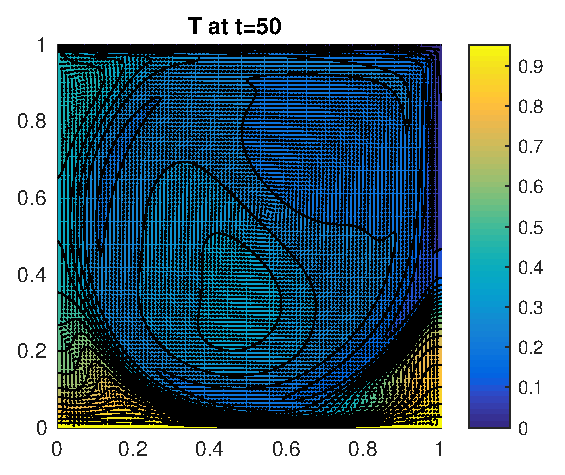
\includegraphics[width=.9\linewidth]{Part1_Case_C_Temp.eps}
\end{minipage}
\caption{Case C: Velocity (left) and temperature (right) profiles at $t = 50$.}
\label{fig:1C}
\end{figure}

As Reynolds number is pushed higher additional vortexes in the lower left and right had corner become apparent in figure \ref{fig:1C}. A boundary layer can also be seen on the driving lid. The temperature field shows majority of the interior of the domain is "mixed".




\newpage
\subsection{Question 1}
\includegraphics[width=\textwidth]{Q1.jpg}

\newpage
\subsection{Question 2}
The two stability conditions for a general 2D advection diffusion problem are stated in equations (\ref{eq:advec}) and (\ref{eq:dif}) and the combined condition includes equations (\ref{eq:dif}) and (\ref{eq:combined}).

\noindent Note: \textit{These equations were derived in lectures and part of the exam so the derivation has been omitted from this report}.

\begin{equation}
\label{eq:advec}
\text{Advection (CFL):  } \sigma_x + \sigma_y \leq 1 
\end{equation}

\begin{equation}
\label{eq:dif}
\text{Diffusion: } \beta_x + \beta_y \leq \frac{1}{2}
\end{equation}

\begin{equation}
\label{eq:combined}
\text{Combined: } \frac{\sigma_x^2}{\beta_x} + \frac{\sigma_y^2}{\beta_y} \leq 2
\end{equation} 

In the case of the non-linear Navier Stokes equations we take $a_x = \max{|u|}$ and $a_y = \max{|v|}$. Furthermore, by assuming $\Delta x = \Delta y = h$, equations (\ref{eq:advec}) - (\ref{eq:combined}) can be further simplified to equations (\ref{eq:dt_CFL}) - (\ref{eq:dt_combined}). A final conservative assumption to equations  (\ref{eq:dt_CFL}) and (\ref{eq:dt_combined}) is that $ \max{|u|} \approx\max{|v|} < U_{lid} = 1$.

\begin{equation}
\label{eq:dt_CFL}
\text{CFL: } \Delta t \leq \frac{h}{\max(|u|) + \max(|v|)}  \approx \frac{h}{2}
\end{equation}

\begin{equation}
\label{eq:dt_diffusion}
\text{Viscous limit: } \Delta t \leq \frac{h^2}{4} \text{Re}
\end{equation}

\begin{equation}
\label{eq:dt_combined}
\text{Combined: } \Delta t \leq \frac{2}{\text{Re} \left(\max(|u|)^2 + \max(|v|)^2\right)}  \approx \frac{1}{Re}
\end{equation}\\




These conditions have been tabulated for cases A - C below:

\begin{center}


\begin{tabular}{c|cc|ccc}

 & Re & h & CFL & Viscous & Combined \\ 
\hline 
Case A  & 20 & $\frac{1}{30}$ & 0.0167 & 0.0056 & 0.05000 \\ 

Case B  & 200  & $\frac{1}{50}$  & 0.0100 & 0.0200& 0.00500  \\ 

Case C & 4000 & $\frac{1}{100}$  & 0.0050 & 0.1000 & 0.00025  \\ 

\end{tabular} 
\end{center}


It can be seen that the energy equation takes a similar form to the momentum equation with the Peclet number replacing the Reynolds number. Hence we can assert the following analogous conditions to equations (\ref{eq:dt_diffusion}) and (\ref{eq:dt_combined}):

\begin{equation}
\text{Viscous: } \Delta t_{energy} \leq \frac{2}{\text{Pe} \left(\max(|u|)^2 + \max(|v|)^2\right)}  \approx \frac{1}{Pe} = \frac{1}{Pr}\Delta t_{momentum}
\end{equation}

\begin{equation}
\label{eq:energy}
\text{Combined: } \Delta t_{energy} \leq \frac{h^2}{4} \text{Pe} = Pr \Delta t_{momentum}
\end{equation}

In the case that $Pr = 0.71 < 1$ then in the viscous limit (equation (\ref{eq:energy}))$\Delta t_{energy} < \Delta t_{momentum}$ is a stricter condition.





\newpage
\subsection{Question 3}
\includegraphics[width=\textwidth]{Q3A.jpg}
\noindent \includegraphics[width=\textwidth]{Q3B.jpg}

This same reasoning can be applied to the 2D problem yielding:
\begin{equation}
\frac{p_{2,j} - p_{1,j} }{\Delta x^2} + \frac{p_{1,j+1} - 2p_{1,j} + p_{1,j-1}}{\Delta y^2}
\end{equation}


\subsection{Question 4}

Figure \ref{fig:timeseries} depicts the velocity measure at a probe in the center of the domain in cases A - C. It can be seen that case A reaches a steady state in under 5 time units whereas case B take between 5 - 10. In the 50 seconds of simulation time it is clear that case C has not yet shown steady state behavior.\\

Qualitatively one can conclude that increasing Reynolds number leads to an increased time to reach a steady state however with only 3 test cases a quantitative relation cannot be obtained. This qualitative relationship makes intuitive sense since at low Reynolds number the Navier-Stokes equation act like the Stokes equations which are parabolic. As Reynolds number increases the flow is dominated by the advection term leading to less diffusive behavior.


\begin{figure}[H]
\centering
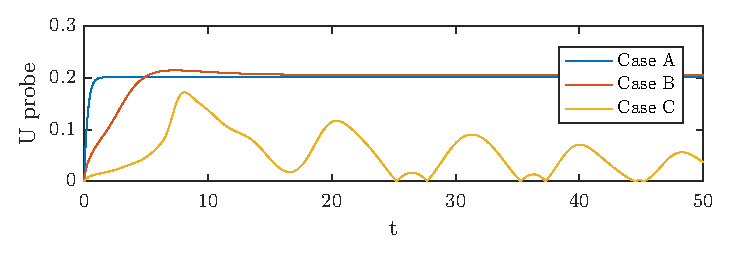
\includegraphics[]{Probe_history.eps}
\caption{Time histories of absolute velocity of a probe located in the center of the domain.}
\label{fig:timeseries}
\end{figure}





\subsection{Question 5}




Figure \ref{fig:OpenFOAM} shows the velocity field obtained in OpenFOAM. The strong resemblance to figure \ref{fig:1C} suggests the Matlab code is somewhat reasonable.

\begin{figure}[h]
\centering
\includegraphics[width=.9\linewidth]{OpenFOAM.png}
\caption{Velocity field of Case C run in OpenFOAM.}
\label{fig:OpenFOAM}
\end{figure}

In order to scrutinize the Matlab code further, figure \ref{fig:Q5} shows the U and V profiles of a vertical slice through $x = 0.5$ at t = 50 for case C as computed with OpenFOAM and the Matlab code. Good agreement can be seen in the U velocity plot which lends validity to the Matlab program. Observing the V velocity a similar trend can be seen however the magnitudes are slightly off. This could be attributed to an number of factors such as differences in numerics however the most likely explanation for this discrepancy is due to transient effects. Figure \ref{fig:timeseries} indicated that at t = 50 the system had not yet reached a steady state and the same can be said about the OpenFOAM results. 

While the close correlation in U profile gives strong evidence as validation to the Matlab code it would be advised to run each simulation to a final steady state to arrive at a more consistent conclusion.


\begin{figure}[H]
\centering
\begin{minipage}{.5\textwidth}
  \centering
  \includegraphics[width=.9\linewidth]{Ucenter.eps}
\end{minipage}%
\begin{minipage}{.5\textwidth}
  \centering
  \includegraphics[width=.9\linewidth]{Vcenter.eps}
\end{minipage}
\caption{U (left) and V (right) profiles at t = 50 along a verticle centerline.}
\label{fig:Q5}
\end{figure}


\newpage
\section{ Rayleigh-Bénard}

\subsection{Case A}

Table \ref{tbl:part2A} outlines the simulation settings for case A of the Rayleigh-Bénard problem. Both the velocity and temperature fields at $t = 20$ are plotted in figure \ref{fig:2A1}.. Finally figure \ref{fig:timeseries_1A} shows a time series of U from a probe in the center of the domain.

 
\begin{table}[H]
\centering
\begin{tabular}{c|cccccccc}
 & Ra & $l_x$ & $l_y$ & $T_{top}$ &$ T_{bottom}$ & $N_x$ & $N_y$ & $\Delta t$ \\ 
\hline 
Case A1 & 200& 10 & 1& 1 & 0  & 200 & 20 & 0.0005 \\ 

Case A2 & 2000 & 10 & 1& 1 & 0  & 200 & 20 & 0.0005 \\ 
 
Case A3 & 60000 & 10 & 1& 1 & 0  & 200 & 20 & 0.0005 \\ 

\end{tabular} 
\caption{Simulation setting for Rayleigh-Bénard Case A.}
\label{tbl:part2A}
\end{table}



\begin{figure}[H]
  \centering
  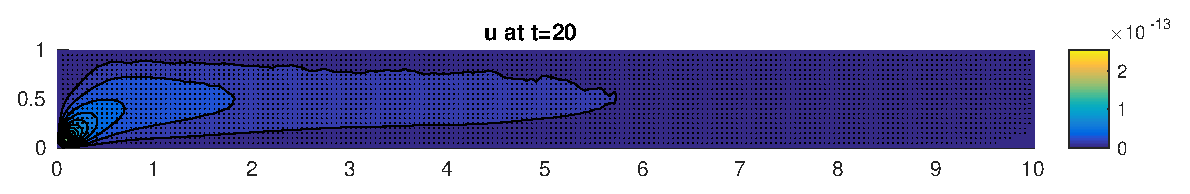
\includegraphics[width=\linewidth]{Part2_Case_A1_Velocity.eps}
  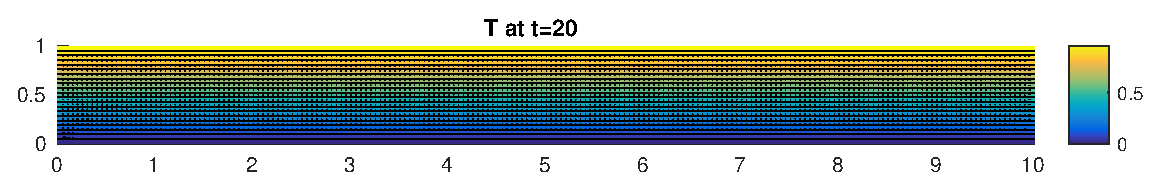
\includegraphics[width=\linewidth]{Part2_Case_A1_Temp.eps}
    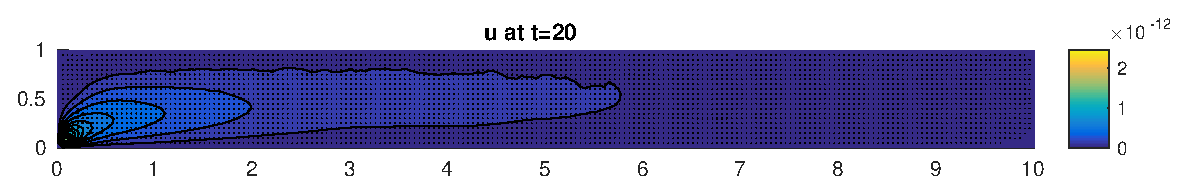
\includegraphics[width=\linewidth]{Part2_Case_A2_Velocity.eps}
  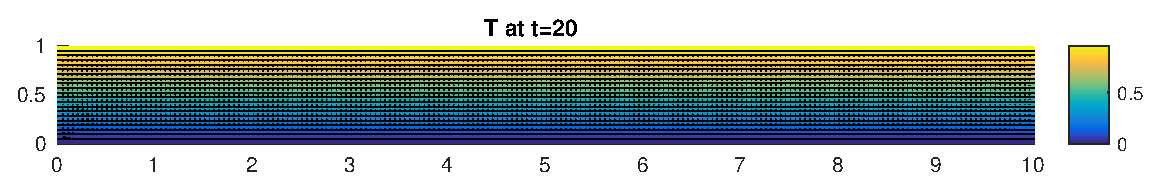
\includegraphics[width=\linewidth]{Part2_Case_A2_Temp.eps}
   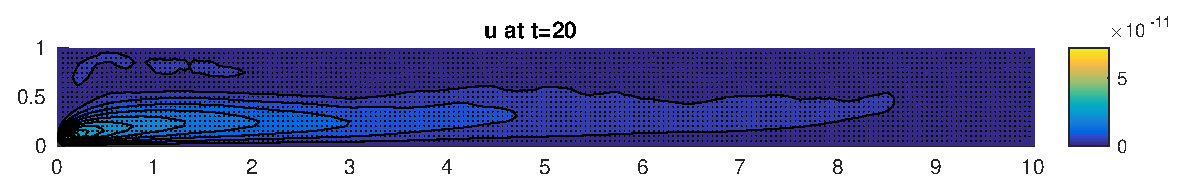
\includegraphics[width=\linewidth]{Part2_Case_A3_Velocity.eps}
  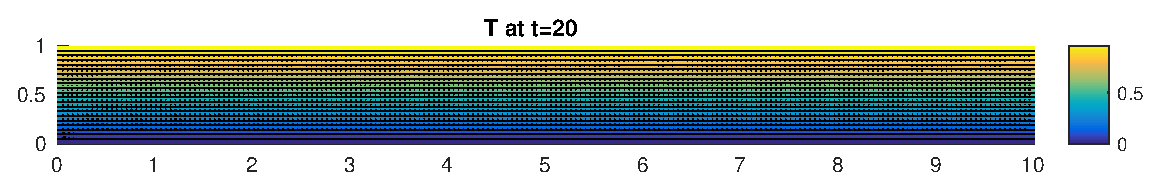
\includegraphics[width=\linewidth]{Part2_Case_A3_Temp.eps}
\caption{Top to bottom: Cases A1 - A3: Rayleigh numbers 200, 2000, 60000. Velocity (top) and temperature (bottom) profiles at $t = 20$.}
\label{fig:2A1}
\end{figure}



\begin{figure}[H]
\centering
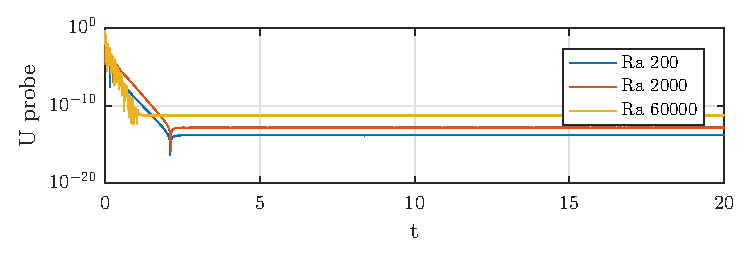
\includegraphics[]{Probe_history2A.eps}
\caption{Time histories of absolute velocity of a probe located in the center of the domain.}
\label{fig:timeseries_1A}
\end{figure}

It can be seen in the above plots that the velocity feilds in all cases are stable, which is to be expcted. In particular figure \ref{fig:timeseries_1A} shows that the initial pertubations are diffused to a steady state. 

\subsection{Case B}

Table \ref{tbl:part2B} outlines the simulation settings for case B of the Rayleigh-Bénard problem. Cases B1 and B2 where chosen by trial and error to determine the critical Rayleigh number. Both the velocity and temperature fields at $t = 20$ are plotted in figure \ref{fig:case2B}. Finally figure \ref{fig:timeseries_1B} shows a time series of U from a probe in the center of the domain.

 
\begin{table}[H]
\centering
\begin{tabular}{c|cccccccc}
 & Ra & $l_x$ & $l_y$ & $T_{top}$ &$ T_{bottom}$ & $N_x$ & $N_y$ & $\Delta t$ \\ 
\hline 
Case A1 & 1710& 10 & 1& 0 & 1  & 200 & 20 & 0.0005 \\ 

Case A2 & 1711 & 10 & 1& 0 & 1  & 200 & 20 & 0.0005 \\ 
 
Case A3 & 1715 & 10 & 1& 0 & 1  & 200 & 20 & 0.0005 \\ 

Case A3 & 5000 & 10 & 1& 0 & 1  & 200 & 20 & 0.0005 \\

\end{tabular} 
\caption{Simulation setting for Rayleigh-Bénard Case A.}
\label{tbl:part2B}
\end{table}

Figure \ref{fig:case2B} shows convection cells in the velocity fields for all cases, with velocity maginitude increasing with increased Rayleigh number. The temperture gradient is slightly disturbed at low Rayleigh number but is more or less the initial linear gradient.

At high Rayleigh number however the convection cells lift the hot fluid at the bottom of the plate up towards the cold plate only for it to cool down and flow to the bottom resulting in what looks like little mushrooms.

\begin{figure}[H]
  \centering
  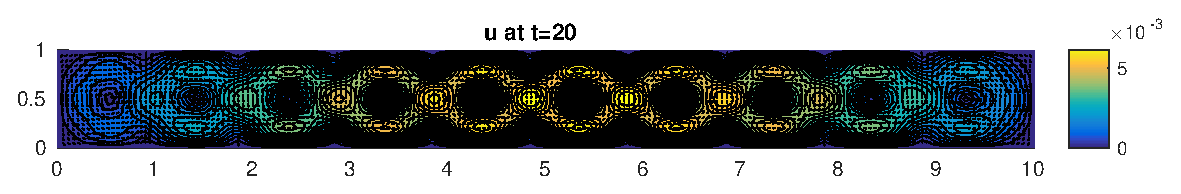
\includegraphics[width=\linewidth]{Part2_Case_B1_Velocity.eps}
  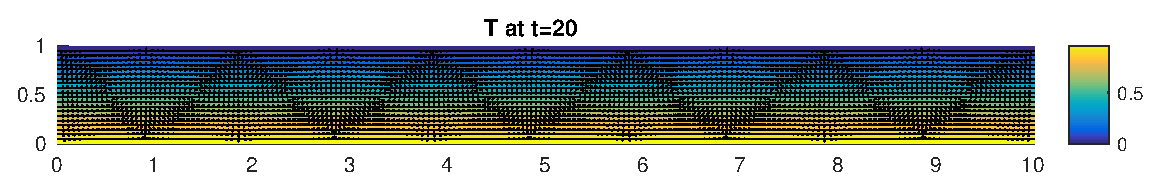
\includegraphics[width=\linewidth]{Part2_Case_B1_Temp.eps}
    \includegraphics[width=\linewidth]{Part2_Case_B2_Velocity.eps}
  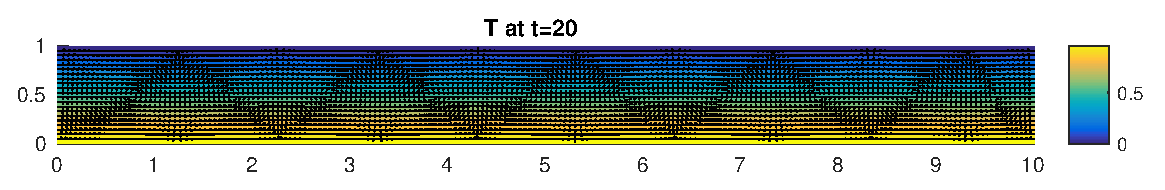
\includegraphics[width=\linewidth]{Part2_Case_B2_Temp.eps}
    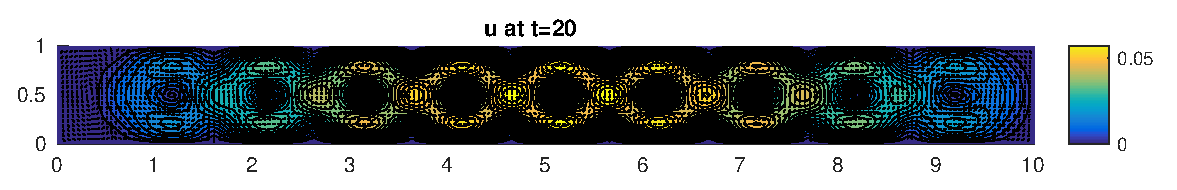
\includegraphics[width=\linewidth]{Part2_Case_B3_Velocity.eps}
  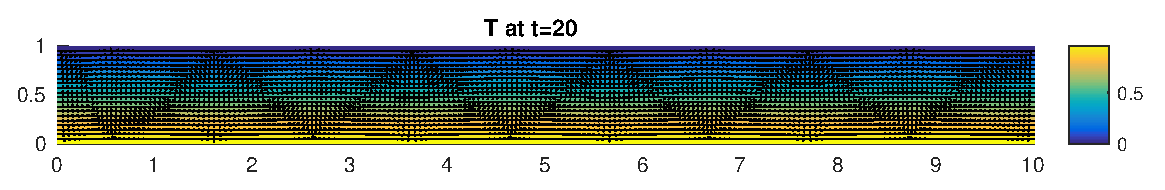
\includegraphics[width=\linewidth]{Part2_Case_B3_Temp.eps}
    \includegraphics[width=\linewidth]{Part2_Case_B4_Velocity.eps}
  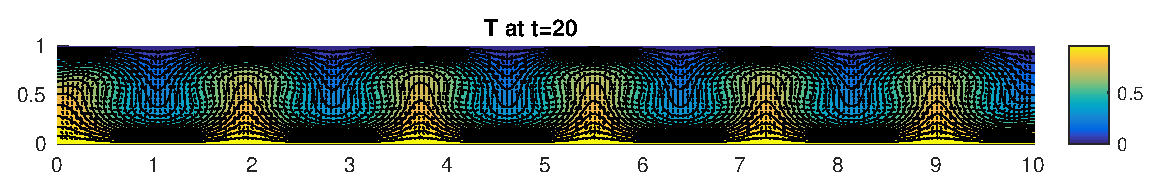
\includegraphics[width=\linewidth]{Part2_Case_B4_Temp.eps}
\caption{Cases B1 - B4: Rayleigh numbers 1710, 1711, 1715 and 5000. Velocity (top) and temperature (bottom) profiles at $t = 20$.}
\label{fig:case2B}
\end{figure}


\newpage
\subsection{Question 1}

Pr. The Prandtl number is the non-dimensional number defined as the ratio between momentum diffusivity and thermal diffusivity, as in equation (\ref{eqn:Pr}). The Prandtl number can be thought of as thermodynamic quantity in the sense that it is dependent on the fluid and the fluid state.
\begin{equation}
\text{Pr} = \frac{\mu \rho}{\kappa/(c_p \rho)} 
\label{eqn:Pr}
\end{equation}
Where $\mu$ is the dynamic viscosity, $\rho$ is the density, $c_p$ is the specific heat and $\kappa$ is the thermal conductivity.\\

\noindent Ra. The Rayleigh number is defined as the ratio of timescales for diffusive thermal transport and convective thermal transport. It should be noted that the convective thermal transport is with respect to some velocity scale $U$. In the context of Rayleigh Bernard convection it is intuitive to think of the Rayleigh number as the balancing of the gravitational force which occurs due to the density gradient between the two plates and the viscous damping in the fluid, as in equation (\ref{eqn:Ra}).
\begin{equation}
\text{Ra} = \frac{g\beta}{\nu \alpha}(T_{bottom} - T_{top})L^3
\label{eqn:Ra}
\end{equation}
Where $g$ is acceleration due to gravity, $\beta$ is the thermal expansion coefficient, $\alpha$ is the thermal diffusivity and $L$ is some characteristic length, in this case the distance between the two plates.\\

\noindent Pe. The Peclet number number is similar to the Reynolds number in the sense that it expresses the ratio between the advection and diffusion of a physical quantity. In the case of heat transfer this quantity is defined in equation (\ref{eqn:Pe}).
\begin{equation}
\text{Pe} = \frac{LU}{\alpha} = \text{Re} \text{Pr}
\label{eqn:Pe}
\end{equation}
\noindent It should be made clear that these three non dimensional quantities along with the Reynolds numbers are not independent of one another. In fact while most of the quantities in equations (\ref{eqn:Pr}) - (\ref{eqn:Pe}) have natural choices in the context of Rayleigh Bernard convection (whether they are thermodynamic properties of the fluid or $L$ being the height of the channel) there is no intuitive choice for a velocity scale $U$. 
With this in mind the entire system can be uniquely defined by:
\begin{itemize}
\item Setting the Prandtl number based entirely on fluid properties.
\item Varying the Rayleigh number to study stability of the system.
\item Setting Pe = 1 analogous to setting a velocity scale in the problem.
\end{itemize} 
Hence the Reynolds number falls out naturally as $\text{Re} = \frac{1}{\text{Pr}}$.

\subsection{Question 2}

Figure \ref{fig:findpeaks} shows a horizontal slice of the velocity magnitude through the domain. It can be seen in this figure that the average half wavelength is 1. hence in this simulation we conclude $\lambda = 2.0$ which is very close to the critical wavelength observed in literature.

End effects can be seen in this plot with wavelength decreasing as the convective currents are squished against the walls. 

In order to exactly represent the critical Rayleigh number one should employ periodic boundary conditions for both velocity and temperature on the left and right hand side. The same Dirichlet boundary conditions on the top and bottom are appropriate. 


\begin{figure}[H]
\centering
\includegraphics[width=\linewidth]{findpeaks.eps}
\caption{Horizontal slice of velocity magnitude for Ra = 1715 indicating peak velocities.}
\label{fig:findpeaks}
\end{figure}

\subsection{Question 3}

Figure \ref{fig:timeseries2} shows that at Ra = 1710 the instabilities will decay exponentially (as indicated by the negative gradient of the velocity probe) while at Re = 1711 exponential growth is observed. This observation is further corroborated in the velocity profiles in figure \ref{fig:case2B} if close attention is payed to the scale of the colour map. Even at time t = 20 a drastic difference between the velocity magnitudes can be seen. 

This leads to the conclusion that the neutrally stable state exists between Ra = 1710 and Ra = 1711 which is close to that observed in literature (Ra = 1708).


\begin{figure}[H]
\centering
\includegraphics[width=\linewidth]{Probe_history2.eps}
\caption{Time history of a central probe comparing cases Ra = 1710 and Ra = 1711. Note the differing y-axis scales used to highlight the gradient of the time series.}
\label{fig:timeseries2}
\end{figure}


\end{document}